\chapter{Planar Graphs}
Ajur was so enamored by Hamiltonian cycles, he was eager to meet Rishnak and
waiting to hear what he is going to talk next. Rishnak was eager to meet Ajur and share about drawing of graphs,=,
A planar graph is a graph that can be drawn such that no edges cross other than at
the vertices. That is there is at least one drawing in which the edges do not cross.
If there is no such drawing available for a graph it is called as non-planar graphs.
For example here are two drawings of a complete graph on Four vertices $K_4$. Since Figure \ref{9g2} has no edge crossing, we can call $K_4$ as a planar graph.
\begin{figure}
\begin{center}
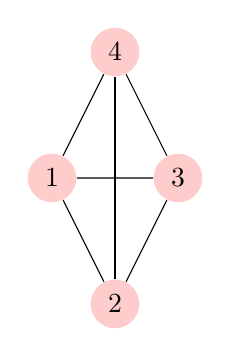
\begin{tikzpicture}
  [scale=.4,auto=left,every node/.style={circle,fill=red!20}]
  \node (n1) at (1,7) {1};
  \node (n2) at (3,3)  {2};
  \node (n3) at (5,7)  {3};
  \node (n4) at (3,11)  {4};

  \foreach \from/\to in {n1/n2,n2/n3,n2/n4,n1/n4,n3/n4,n1/n3}
    \draw (\from) -- (\to);

\end{tikzpicture}
\caption{ Drawing of $K_4$ in which edges cross}\label{9g1}
\end{center}
\end{figure}
\begin{figure}
\begin{center}
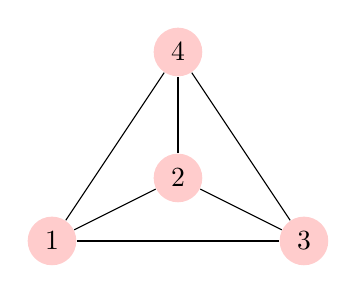
\begin{tikzpicture}
  [scale=.4,auto=left,every node/.style={circle,fill=red!20}]
  \node (n1) at (-1,7) {1};
  \node (n2) at (3,9)  {2};
  \node (n3) at (7,7)  {3};
  \node (n4) at (3,13)  {4};

  \foreach \from/\to in {n1/n2,n2/n3,n2/n4,n1/n4,n3/n4,n1/n3}
    \draw (\from) -- (\to);

\end{tikzpicture}
\caption{ Planar Drawing of $K_4$}\label{9g2}
\end{center}
\end{figure}
 Rishnak showed another graph \ref{9g3} asked Ajur whether he can draw with no edges crossing.
 \begin{figure}
\begin{center}
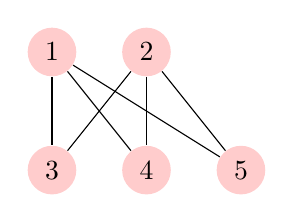
\begin{tikzpicture}
  [scale=.3,auto=left,every node/.style={circle,fill=red!20}]
  \node (n1) at (1,7) {1};
  \node (n2) at (5,7)  {2};
  \node (n3) at (1,2)  {3};
  \node (n4) at (5,2) {4};
  \node (n5) at (9,2)  {5};
 
  
   \foreach \from/\to in {n1/n3,n1/n4,n1/n5,n2/n3,n2/n4,n2/n5}
    \draw (\from) -- (\to);
    \end{tikzpicture}
\caption{ A Bipartite Graph with 5 vertices and 6 edges, denoted by $K_{2,3}$ where the edges cross}\label{9g3}
\end{center}
\end{figure}
Ajur thought for a while and found it a bit challenging. Then he thought of moving the vertex 2 down in which case no edges will cross. He drew the graph as shown in Figure \ref{9g4}
\begin{figure}
\begin{center}
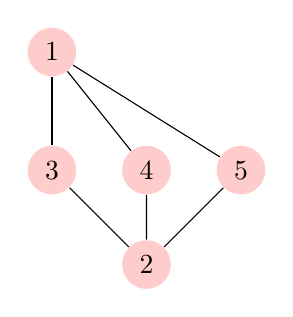
\begin{tikzpicture}
  [scale=.3,auto=left,every node/.style={circle,fill=red!20}]
  \node (n1) at (1,7) {1};
  \node (n2) at (5,-2)  {2};
  \node (n3) at (1,2)  {3};
  \node (n4) at (5,2) {4};
  \node (n5) at (9,2)  {5};
 
  
   \foreach \from/\to in {n1/n3,n1/n4,n1/n5,n2/n3,n2/n4,n2/n5}
    \draw (\from) -- (\to);
    \end{tikzpicture}
\caption{ Planar Drawing of a Bipartite Graph ($K{2,3}$ with 5 vertices and 6 edges with  no edge crossing}\label{9g4}
\end{center}
\end{figure}

Rishnak was impressed. Rishnak then asked Ajur to find out whether this graph \ref{9g5} has a plane representation. Ajur struggled and tried to get a drawing - with one edge crossing \ref{9g6}. 

\begin{figure}
\begin{center}
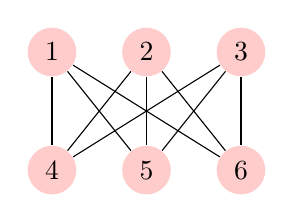
\begin{tikzpicture}
  [scale=.3,auto=left,every node/.style={circle,fill=red!20}]
  \node (n1) at (1,7) {1};
  \node (n2) at (5,7)  {2};
  \node (n3) at (9,7) {3};
  \node (n4) at (1,2)  {4};
  \node (n5) at (5,2) {5};
  \node (n6) at (9,2)  {6};
 
  
   \foreach \from/\to in {n1/n6,n1/n4,n1/n5,n2/n6,n2/n4,n2/n5,n3/n4,n3/n5,n3/n6}
    \draw (\from) -- (\to);
    \end{tikzpicture}
\caption{ A Bipartite Graph with 6 vertices and 9 edges, denoted by $K_{3,3}$ where the edges cross}\label{9g5}
\end{center}
\end{figure}
\begin{figure}
\begin{center}
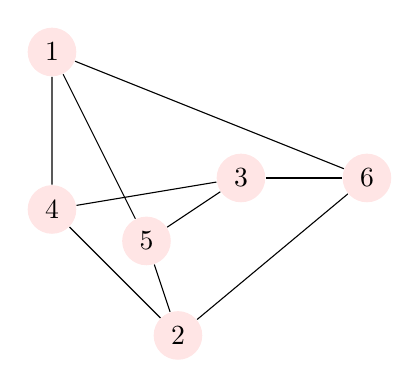
\begin{tikzpicture}
  [scale=.4,auto=left,every node/.style={circle,fill=red!10}]
  \node (n1) at (1,7) {1};
  \node (n2) at (5,-2)  {2};
  \node (n3) at (7,3) {3};
  \node (n4) at (1,2)  {4};
  \node (n5) at (4,1) {5};
  \node (n6) at (11,3)  {6};
 
  
   \foreach \from/\to in {n1/n6,n1/n4,n1/n5,n2/n6,n2/n4,n2/n5,n3/n4,n3/n5,n3/n6}
    \draw (\from) -- (\to);
    \end{tikzpicture}
\caption{ A  drawing of Bipartite Graph with 6 vertices and 9 edges, denoted by $K_{3,3}$ where just two edges edges cross}\label{9g6}
\end{center}
\end{figure}
Rishnak told Ajur that this graph does not have a planar representation. He added that this is a well known puzzle due to Sam Loyd\footnote{Sam Lloyd is a famous American Recreational Mathematician who has contributed a lot of puzzles}. There are three houses (represented as circles) drawn on paper and below them three smaller circles representing gas, water, and electricity suppliers. The aim of the puzzle is to draw lines to get each utility into every house, without crossing over any line. Ajur reminded himself that he should read up on Loyd's puzzle books from his local library.

 Rishnak asked Ajur if two graphs $G$ and $H$ are isomorphic and if $G$ is planar, can you say $H$ is planar. Ajur said if $H$ is isomorphic to $G$, then each vertex corresponds to some vertex of $G$. By just relabeling the vertices of $G$ in its planar drawing, we get a planar drawing of $H$.
 
 Ajur then excitedly told Risnak that all trees have a planar representation\footnote{Ajur liked monkeys and monkeys liked trees.}. Rishnak answered that trees are easy to embed in a plane as there are
 no cycles. He added that there is a nice space filling planar representation of a tree shown in Figure \ref{9g7}.
\begin{figure}
\begin{center}    

 \begin{tikzpicture}[decoration=H-tree, very thick]
    \draw decorate { decorate { decorate { decorate { decorate { decorate { (0,0) -- (3,0) }}}}}};
  \end{tikzpicture}
  \caption{ A planar drawing of a tree (which is self similar)}\label{9g7}
  \end{center}
\end{figure}

One way to get a planar drawing is to embed the longest cycle in a planar and then try to place the rest of the vertices so that there are no edges cross each other. This cycle will divide the plane into two region inner region (inside the cycle) or outer region (outside the cycle). So the edges have to go either inside or outside. By trying out the possibilities, you can get a planar representation of a graph (if it exists). It is easier than done. One can do an efficient method of placing the edges (without any backtracking) - Rishnak said some details are more complicated. 

Each region in a planar representation is also called a face. Euler discovered a remarkable formula concerning the number of edges, e, the number of vertices,n, and the number of faces, f as,
\begin{equation}
\label{eqn:euler}
  f-e+v=2 
\end{equation}

 

Rishnak gave an intuitive explanation of this formula \ref{eqn:euler}. Since each region is a cycle and the external region (sometimes called an infinite region) is also a cycle. There are \ref{eqn:cycles} $n-1$ edges in a tree, the rest of $e-(n-1)$ edges will form a cycle. Each of these cycles correspond to an internal region or internal face, and there is one external face. Hence from \ref{eqn:cycles}, Euler's equation \ref{eqn:euler} folows.
\begin{eqnarray*}
    \label{eqn:cycles}
    internal faces&=&e-(n-1)\\
    external face&=&1\\
    total faces&=& internal faces~+~external face\\
    &=&e-n+2
\end{eqnarray*}

Ajur told Rishnak that he has done Platonic solids with Zometools \footnote{Zometool is a commercial kit to make polyhedrons}. Rishnak then explained Euler's equation applied for the five platonic solids by the following table \ref{tab:platonic} where $n$ stands for the number of vertices, $e$ stands for the number of edges and $f$ stands for the number of faces. All Platonic solids have a planara representation.
\begin{table}[]
    \centering
    \begin{tabular}{||c|c|c|c||}
    \hline
    Solid & n & e& f \\ [0.5ex] 
 \hline\hline
 Tetrahedron& 4 & 6 & 4 \\ 
 \hline
 Octohedron & 6 & 12& 8 \\
 \hline
 Cube & 8 & 12 & 6 \\
 \hline
 Dodecahedron & 20 & 30 & 12 \\
 \hline
 Icosahedron & 12 & 30 & 20 \\ [1ex] 
 \hline
 \end{tabular}
    \caption{Euler Equation for Platonic Solids}
    \label{tab:platonic}
\end{table}


that  Rishnak said another interesting fact (without further details) that any planar graph has not only a plane representation but also a representation in which